%% LyX 2.3.7 created this file.  For more info, see http://www.lyx.org/.
%% Do not edit unless you really know what you are doing.
\documentclass[10pt,english,t,10pt]{beamer}
\usepackage{lmodern}
\usepackage[T1]{fontenc}
\usepackage[utf8]{inputenc}
\setcounter{tocdepth}{1}
\setlength{\parskip}{\smallskipamount}
\setlength{\parindent}{0pt}
\usepackage{units}
\usepackage{amstext}
\usepackage{amssymb}
\usepackage{graphicx}
\usepackage[authoryear]{natbib}
\PassOptionsToPackage{normalem}{ulem}
\usepackage{ulem}

\makeatletter
%%%%%%%%%%%%%%%%%%%%%%%%%%%%%% Textclass specific LaTeX commands.
% this default might be overridden by plain title style
\newcommand\makebeamertitle{\frame{\maketitle}}%
% (ERT) argument for the TOC
\AtBeginDocument{%
  \let\origtableofcontents=\tableofcontents
  \def\tableofcontents{\@ifnextchar[{\origtableofcontents}{\gobbletableofcontents}}
  \def\gobbletableofcontents#1{\origtableofcontents}
}

%%%%%%%%%%%%%%%%%%%%%%%%%%%%%% User specified LaTeX commands.



\usepackage{tikz}
\usetikzlibrary{positioning}
\usepackage{appendixnumberbeamer}

\usepackage{graphicx}
\usepackage{subfig}

\usetheme[progressbar=frametitle,block=fill,subsectionpage=progressbar]{metropolis}

% margin
\setbeamersize{text margin right=1.5cm}

% colors
\definecolor{DarkRed}{rgb}{0.7,0,0}
%\colorlet{DarkRed}{red!70!black}
\setbeamercolor{normal text}{fg=black}
\setbeamercolor{alerted text}{fg=DarkRed}
\setbeamercolor{progress bar}{fg=DarkRed}
\setbeamercolor{button}{bg=DarkRed}

% width of seperators
\makeatletter
\setlength{\metropolis@titleseparator@linewidth}{1pt}
\setlength{\metropolis@progressonsectionpage@linewidth}{1pt}
\setlength{\metropolis@progressinheadfoot@linewidth}{1pt}
\makeatother

% new alert block
\newlength\origleftmargini
\setlength\origleftmargini\leftmargini
\setbeamertemplate{itemize/enumerate body begin}{\setlength{\leftmargini}{4mm}}
\let\oldalertblock\alertblock
\let\oldendalertblock\endalertblock
\def\alertblock{\begingroup \setbeamertemplate{itemize/enumerate body begin}{\setlength{\leftmargini}{\origleftmargini}} \oldalertblock}
\def\endalertblock{\oldendalertblock \endgroup}
\setbeamertemplate{mini frame}{}
\setbeamertemplate{mini frame in current section}{}
\setbeamertemplate{mini frame in current subsection}{}
\setbeamercolor{section in head/foot}{fg=normal text.bg, bg=structure.fg}
\setbeamercolor{subsection in head/foot}{fg=normal text.bg, bg=structure.fg}

% footer
\makeatletter
\setbeamertemplate{footline}{%
    \begin{beamercolorbox}[colsep=1.5pt]{upper separation line head}
    \end{beamercolorbox}
    \begin{beamercolorbox}{section in head/foot}
      \vskip1pt\insertsectionnavigationhorizontal{\paperwidth}{}{\hskip0pt plus1filll \insertframenumber{} / \inserttotalframenumber \hskip2pt}\vskip3pt% 
    \end{beamercolorbox}%
    \begin{beamercolorbox}[colsep=1.5pt]{lower separation line head}
    \end{beamercolorbox}
}
\makeatother

% toc
\setbeamertemplate{section in toc}{\hspace*{1em}\inserttocsectionnumber.~\inserttocsection\par}
\setbeamertemplate{subsection in toc}{\hspace*{2em}\inserttocsectionnumber.\inserttocsubsectionnumber.~\inserttocsubsection\par}


% Automatically create vspace between items
% See: https://tex.stackexchange.com/questions/369504/beamer-vertically-stretching-level-1-list-items-in-a-nested-list-environment
%\usepackage{xpatch} 
%\xpatchcmd{\itemize}   
%	{\def\makelabel}   
%	{\ifnum\@itemdepth=1\relax      
%		\setlength\itemsep{\fill} % separation for first level    
%		\fi\def\makelabel   
%	}{}{} 
%\xpatchcmd{\enditemize}   
%	{\endlist}   
%	{\endlist\ifnum\@itemdepth<2\else\vfil\fi}{}{}




% Automatically create vspace between items
% See: https://jayrobwilliams.com/posts/2019/10/better-beamer
\makeatletter
\renewcommand{\itemize}[1][]{%
  \beamer@ifempty{#1}{}{\def\beamer@defaultospec{#1}}%
  \ifnum \@itemdepth >2\relax\@toodeep\else
    \advance\@itemdepth\@ne
    \beamer@computepref\@itemdepth% sets \beameritemnestingprefix
    \usebeamerfont{itemize/enumerate \beameritemnestingprefix body}%
    \usebeamercolor[fg]{itemize/enumerate \beameritemnestingprefix body}%
    \usebeamertemplate{itemize/enumerate \beameritemnestingprefix body begin}%
    \list
      {\usebeamertemplate{itemize \beameritemnestingprefix item}}
      {\def\makelabel##1{%
          {%
            \hss\llap{{%
                \usebeamerfont*{itemize \beameritemnestingprefix item}%
                \usebeamercolor[fg]{itemize \beameritemnestingprefix item}##1}}%
          }%
        }%
      }
  \fi%
  \setlength\itemsep{\fill}
    \ifnum \@itemdepth >1
        \vfill
    \fi%  
  \beamer@cramped%
  \raggedright%
  \beamer@firstlineitemizeunskip%
}

\def\enditemize{\ifhmode\unskip\fi\endlist%
  \usebeamertemplate{itemize/enumerate \beameritemnestingprefix body end}
  \ifnum \@itemdepth >1
        \vfil
  \fi%  
  }
\makeatother

\makeatother

\usepackage{babel}
\begin{document}
\title{2. Consumption-Saving Models \vspace{-2mm}}
\subtitle{Adv. Macro: Heterogenous Agent Models} 
\author{Nicolai Waldstrøm}
\date{2024}

{
\setbeamertemplate{footline}{} 
\begin{frame}

\maketitle

\begin{tikzpicture}[overlay, remember picture]
\node[above left=0cm and 0.0cm of current page.south east] 
{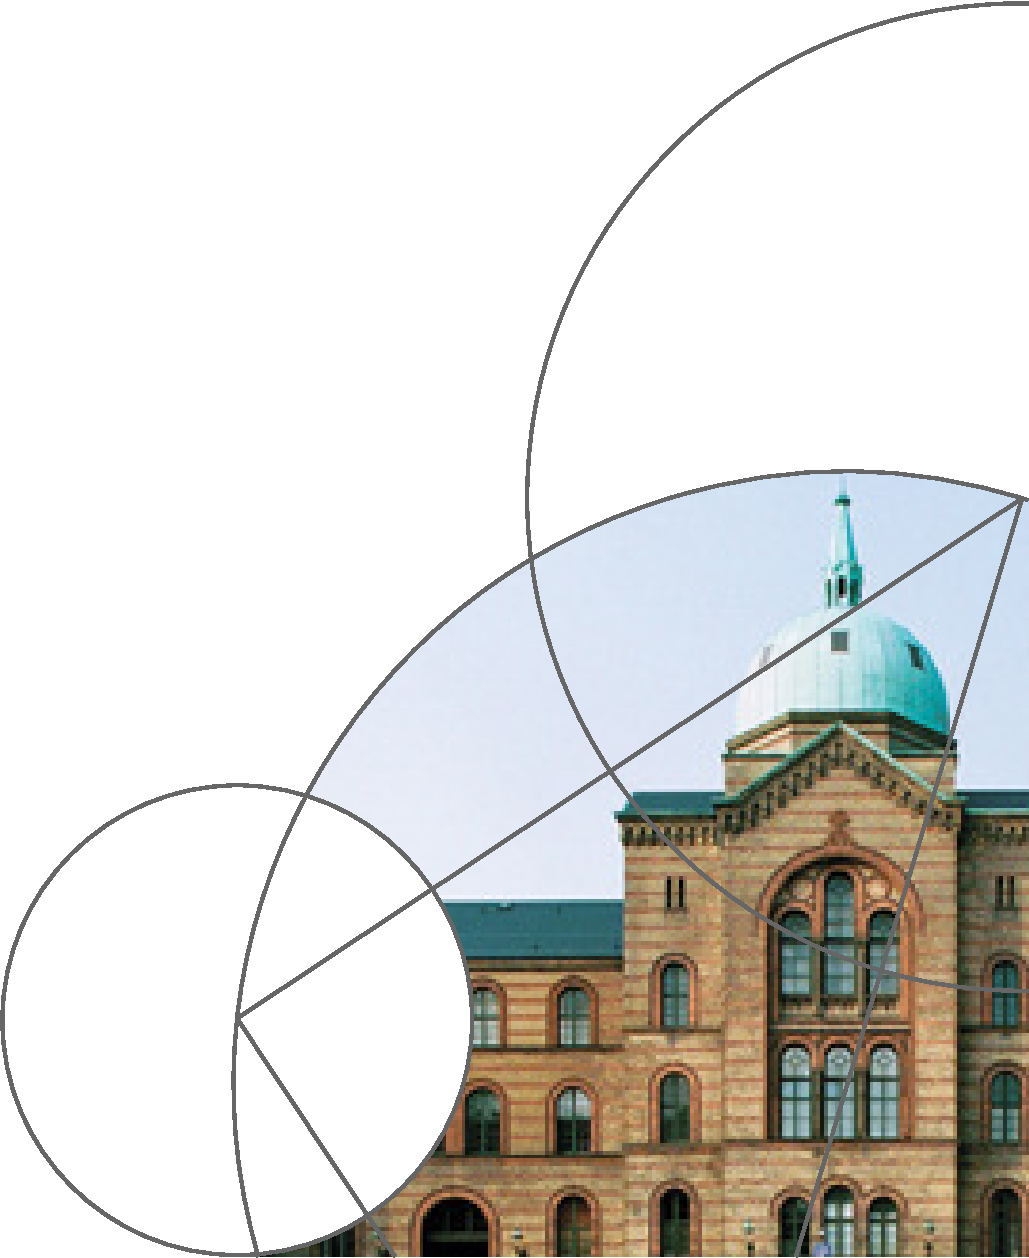
\includegraphics[width=4cm]{figs/KUSAMFtitlelrcorner.pdf}};
\end{tikzpicture}

\begin{tikzpicture}[overlay, remember picture]
\node[below left=0.5cm and .8cm of current page.north east] 
{\includegraphics[width=1.5cm]{figs/KUSAMFlogo.pdf}};
\end{tikzpicture}


\end{frame}
}

\addtocounter{framenumber}{-1}


\section{Advertisement}
\begin{frame}{Cagé and Piketty at CSS}

\begin{columns}[T] % Left column for text and bullets         
\begin{column}{0.6\textwidth}             
\begin{itemize}                 
\item Thomas Piketty and Julia Cagé will visit CSS and discuss \textbf{the history of policy conflict  }              
\item October 10 at 17:00-18:00 in room 35.01.05              
\item Interview by editor at danish newspaper \textit{Information}, Rune Lykkeberg                
\item The first 100 students who sign-up will be able to attend (\href{https://forms.office.com/pages/responsepage.aspx?id=S9iZHj8WBU20AwL9yXLYCrLwJkQ6_BhEvvpwBS_0JANUQlVPNzlNMkpRVDk3TTlaNUxFWjcxNlpIOS4u&route=shorturl}{\textcolor{red}{signup link}})            
\end{itemize}         
\end{column}  % Right column for image         
\begin{column}{0.4\textwidth}   
\centering 
\includegraphics[width=\textwidth]{figs/piketty_cage.png} % Replace with your image file         
\end{column}     
\end{columns}
\end{frame}
%

\section{Introduction}
\begin{frame}{Consumption-Saving Models}
\vspace{-2mm}
\begin{itemize}
\item <+->\textbf{Last time: }How to solve consumption-saving models using
dynamic programing 
\item <+->\textbf{Goal for today: }Better understanding of household spending
through the lens of traditional consumption-saving models 
\item <+->\textbf{Central economic questions:}
\begin{enumerate}
\item How do households consume out of transitory income shocks?
\item How to design models that match the empirical evidence on the Marginal
Propensity to Consume (MPC)?
\item What is the effect of income risk on consumption dynamics? \vfill
\end{enumerate}
\item <+->\textbf{Plan for today:}
\begin{enumerate}
\item Discuss the MPC, why it matters, and how it looks in the data
\item Consider a variety of models that attempt to match the data
\item Study the link between income risk and consumption behavior
\end{enumerate}
\item <+->Primarily \textbf{partial equilibrium }- leave general equilibrium
for next lecture\textbf{ }
\end{itemize}
\end{frame}
%

\section{MPC}
\begin{frame}{The Marginal Propensity to Consume (MPC)}
\begin{itemize}
\item <+->\textbf{Definition:} How much a household spends out of a small,
one-time, unanticipated income shock
\end{itemize}
\[
MPC=\frac{\Delta C}{\Delta Y}
\]

\begin{itemize}
\item <+->\textbf{Notes:}
\begin{enumerate}
\item It is the MPC out of a transitory income shock (Friedman, 1957) 
\item It is the contemporaneous MPC (usually one quarter or a year)
\item It is measured based on spending on nondurables and services
\end{enumerate}
\item <+->For a comprehensive overview, see Kaplan and Violante (2022) 
\end{itemize}
\end{frame}
%
\begin{frame}{Why do we care about the MPC?}

\begin{itemize}
\item <+->Central concept in modern heterogeneous-agent macroeconomics 
\item <+->Affects macro response to:
\begin{itemize}
\item Fiscal stimulus
\item Monetary policy
\item Redistribution 
\item External shocks (markup shocks, oil/energy shocks, capital flows)
\end{itemize}
\item <+->Historically: Tension between data and models
\item <+->We need macro models that can reproduce the data on MPC
\end{itemize}
\end{frame}
%
\begin{frame}{MPC in the Data: Methods }
\begin{itemize}
\item Three strands of empirical evidence on the size of the MPC: \vspace{5mm}
\begin{enumerate}
\item <+->Quasi-experimental evidence \\
Johnson-Parker-Souleles (2006): Income tax rebates \\
Gelman et al. (2020): government shutdown \\
Fagereng et al. (2020), Golosov et al. (2021): lottery wins\vspace{5mm}
\item <+->Self-reported MPC from survey questions \\
Bunn et al. (2018), Christelis et al. (2018), Fuster et al. (2020)
\vspace{5mm}
\item <+->Structural estimates \\
Blundell-Pistaferri-Preston (2008), Commault (2019)
\end{enumerate}
\end{itemize}
\end{frame}
%
\begin{frame}{MPC in the Data: Findings}
\begin{itemize}
\item <+->The quarterly aggregate MPC is between 15\% and 25\% 
\begin{itemize}
\item Annual MPCs are larger since spending responses are \emph{persistent}
\item <+->Size dependence: MPC larger for small income shocks 
\item <+->Sign asymmetry: MPC much larger for negative income shocks 
\end{itemize}
\item <+->There is large heterogeneity in MPCs across households 
\begin{itemize}
\item Liquid wealth: MPC larger for low wealth households 
\item Fixed individual characteristics: MPC larger for young, low-income
households
\end{itemize}
\end{itemize}
\end{frame}
%
\begin{frame}{Taking Stock}
\begin{itemize}
\item <+->In the data, the MPC is large and heterogeneous
\item <+->These observations have important implications for modern macro
\item <+->Question: how can common macro models generate a large MPC?
\end{itemize}
\end{frame}
%

\section{MPCs in Macro Models}
\begin{frame}{Model overview}
 
\begin{enumerate}
\item Permanent income hypothesis\\
Friedman (1957)
\item Buffer-stock consumption model \\
Deaton (1991, 1992); Carroll (1992, 1997)
\item Multiple-asset buffer-stock consumption models\\
Kaplan and Violante (2014)
\end{enumerate}
\end{frame}
%
\begin{frame}{Quick aside: General vs. partial equilibrium}
\begin{itemize}
\item <+->Today everything is gonna be set in \textbf{partial equilibrium}
\begin{itemize}
\item No market clearing (labor market, goods market, asset market)
\item Prices $w,r$ are therefore \textbf{exogenous}
\item Only endogenous variables are the choice variables and endo. states
of households
\item Typically consumption $c$ and savings $a$
\end{itemize}
\item <+->General equilibrium
\begin{itemize}
\item Households, firms and government interact through \textbf{market clearing }
\item Prices are endogenous and adjust to clear these markets
\item \textbf{Next lecture}
\end{itemize}
\end{itemize}
\end{frame}
%
\begin{frame}{Representative Agent (RA) Model}
\begin{itemize}
\item No idiosyncratic risk, no borrowing constraint
\item <+->Household problem:
\end{itemize}
\[
\begin{aligned}\max_{\left\{ c_{t},a_{t}\right\} } & \sum_{t=0}^{\infty}\beta^{t}\frac{c_{t}^{1-\sigma}}{1-\sigma}\\
\text{ s.t. }\\
c_{t}+a_{t}= & Ra_{t-1}+y_{t}
\end{aligned}
\]

\begin{itemize}
\item <+->Consumption function:
\[
c\left(a\right)=\mathfrak{m}\left[Ra+\sum_{t=0}^{\infty}\left(\frac{1}{R}\right)^{t}y_{t}\right],\;where\;\mathfrak{m}=1-R^{-1}(R\beta)^{\frac{1}{\sigma}}
\]
\item <+->Observation: The consumption function is linear in asset holdings
$\rightarrow$ wealth distribution irrelevant for MPC\\
$\Rightarrow$ Cannot reproduce empirical evidence on correlation
between wealth and MPCs
\end{itemize}
\end{frame}
%
\begin{frame}{Representative Agent (RA) Model}
\begin{itemize}
\item Parameterization:
\begin{enumerate}
\item Log utility ($\sigma=1$): then we can simplify to: $\mathfrak{m}=1-\beta=r$
\item Plausible (quarterly) calibrations: $\mathfrak{m}=0.5\%$ 
\end{enumerate}
\item <+->Representative Agent model features a tiny MPC
\item <+->Why? With concave utility $u\left(c\right)$ across periods households
want to smooth consumption across periods 
\begin{itemize}
\item <+->I.e. Prefer $u\left(1\right)+\beta u\left(1\right)$ to $u\left(2\right)+\beta u\left(0\right)$
when $\beta$ is high (Jensen's inequality)
\item <+->In the RA model there is nothing preventing excessive consumption
smoothing 
\item <+->Household optimally spread out spending out of income gain across
all periods $\Rightarrow$ low MPC
\end{itemize}
\end{itemize}
\end{frame}
%
\begin{frame}{Main Takeaways for the MPC}

Can macro models generate a high MPC, and if so, how?
\begin{enumerate}
\item RA model: No 
\end{enumerate}
\end{frame}
%
\begin{frame}{One-Asset Heterogeneous Agent (HA) Model}
\begin{itemize}
\item Add idiosyncratic income risk, realistic borrowing constraint
\item <+->Household problem:
\[
\begin{aligned}\max_{\left\{ c_{t},a_{t}\right\} }\mathbb{E}_{0} & \sum_{t=0}^{\infty}\beta^{t}\frac{c_{t}^{1-\sigma}}{1-\sigma}\\
\text{ s.t. }\\
c_{t}+a_{t} & =Ra_{t-1}+y_{t}\\
y_{t+1} & \sim\mathcal{F}(y_{t})\\
a_{t} & \geq0
\end{aligned}
\]
\item <+->Main takeaways:
\begin{enumerate}
\item Consumption function $c\left(a\right)$ is concave due to precautionary
motive
\item There is an optimal buffer stock of assets that HHs want to achieve
\end{enumerate}
\end{itemize}
\end{frame}
%
\begin{frame}{Consumption function is concave}

\centering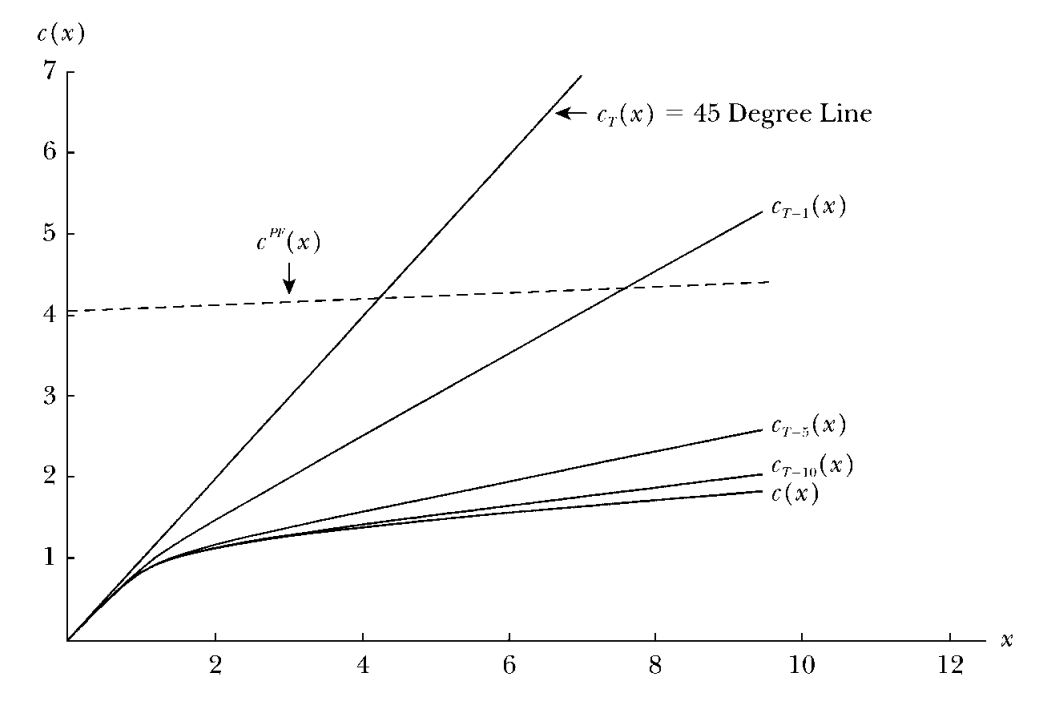
\includegraphics[width=0.6\paperwidth]{figs/consumption-function}
\begin{itemize}
\item $x=\nicefrac{a}{y}$ is the share of assets to permanent income (Carroll
2001)
\item Concavity: Slope of consumption (=MPC) increases as $x\rightarrow0$
\item But approximately linear for large $x$ (as in representative agent
model)
\end{itemize}
\end{frame}
%
\begin{frame}{Households try to achieve an optimal buffer stock}

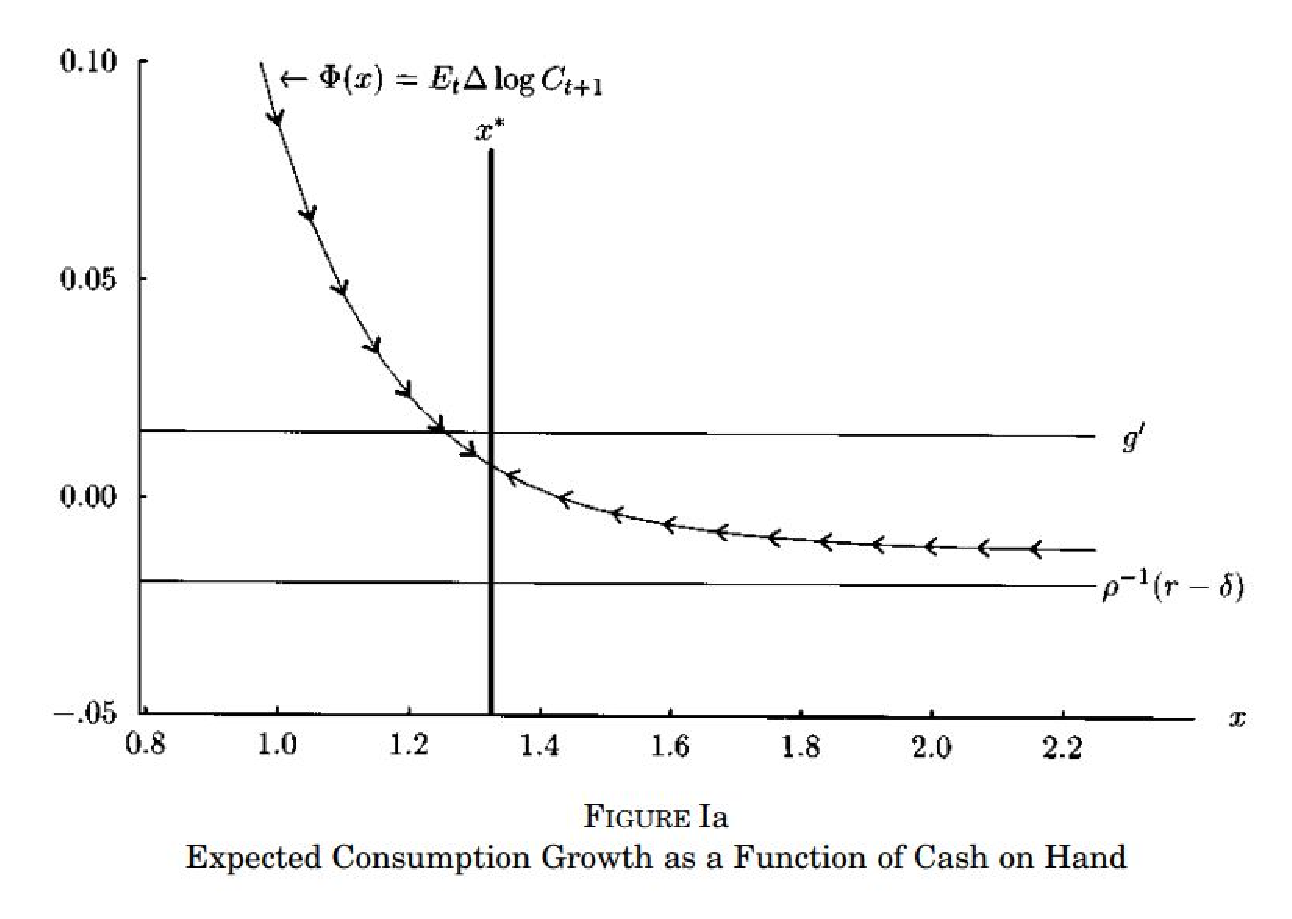
\includegraphics[width=0.6\paperwidth]{figs/buffer-stock-saving}
\begin{itemize}
\item If $x_{t}<x^{*}:$ Expected consumption growth decreases (precautionary
saving motive)
\item If $x_{t}>x^{*}:$ Expected consumption growth increases (impatience,
$\beta R<1$)
\end{itemize}
\end{frame}
%
\begin{frame}{Households try to achieve an optimal buffer stock}

Takeaways:
\begin{enumerate}
\item <+->As $x\rightarrow\infty$, the expected growth rate of consumption
(and the MPC) converge to their values in the RA model
\item <+->As $x\rightarrow0$ the MPC approaches due to binding borrowing
constraint 
\item <+->If the consumer is impatient, there exists a unique target assets-to-permanent-income
ratio ($x^{*}$) 
\end{enumerate}
\end{frame}
%
\begin{frame}{From the inidividual to the aggregate MPC}
\begin{itemize}
\item <+->Individual MPC for a household with state $(a,y)$:
\end{itemize}
\[
m(a,y)=\frac{c(a+x,y)-c(a,y)}{x}\simeq\frac{\partial c(a,y)}{\partial a}
\]

\begin{itemize}
\item <+->Aggregate MPC:
\[
\overline{\mathrm{m}}=\sum_{a,y}\mathfrak{m}(a,y)\times D\left(a,y\right)
\]
\item <+->Two key determinants:
\begin{enumerate}
\item Consumption function $c(a,y)$$\Longrightarrow$MPC function $m(a,y)$
\item Wealth distribution $D(a,y)$
\end{enumerate}
\end{itemize}
\end{frame}
%
\begin{frame}{What determines the size of the aggregate MPC?}
\begin{itemize}
\item <+->Shape of the consumption function $m(a,y)$
\begin{itemize}
\item <+->Uninsurable income risk $\rightarrow$ precautionary saving motive 
\begin{itemize}
\item Risk-aversion and prudence ($u''$,$u'''$) 
\item Occasionally binding borrowing constraint 
\end{itemize}
\item <+->Strength of precautionary saving is decreasing in wealth 
\item <+->Consumption function is concave $\rightarrow$ MPC is decreasing
in wealth 
\item <+->As wealth grows, the MPC $\rightarrow$ MPC in the RA model
\end{itemize}
\item <+->Shape of the wealth distribution $D\left(a,y\right)$
\begin{itemize}
\item Bigger mass at bottom, where $c$ function is concave $\rightarrow$
large MPC
\end{itemize}
\end{itemize}
\end{frame}
%
\begin{frame}{What is a reasonable calibration of such a model?}
\begin{itemize}
\item <+->\textbf{Calibration Strategy:}
\begin{enumerate}
\item As before, we set $\sigma=1$, so that we have log utility
\item Set the interest rate $r$ to be 1\% per year
\item Choose $\beta$ so that the model matches some target of mean wealth 
\end{enumerate}
\item <+->\textbf{Calibration 1:}
\begin{enumerate}
\item Target US data: wealth to income ratio of 4.1
\item This gives an MPC of 4.6\%
\end{enumerate}
\end{itemize}
\end{frame}
%
\begin{frame}{What is a reasonable calibration of such a model?}
\begin{center}
\textbf{\centering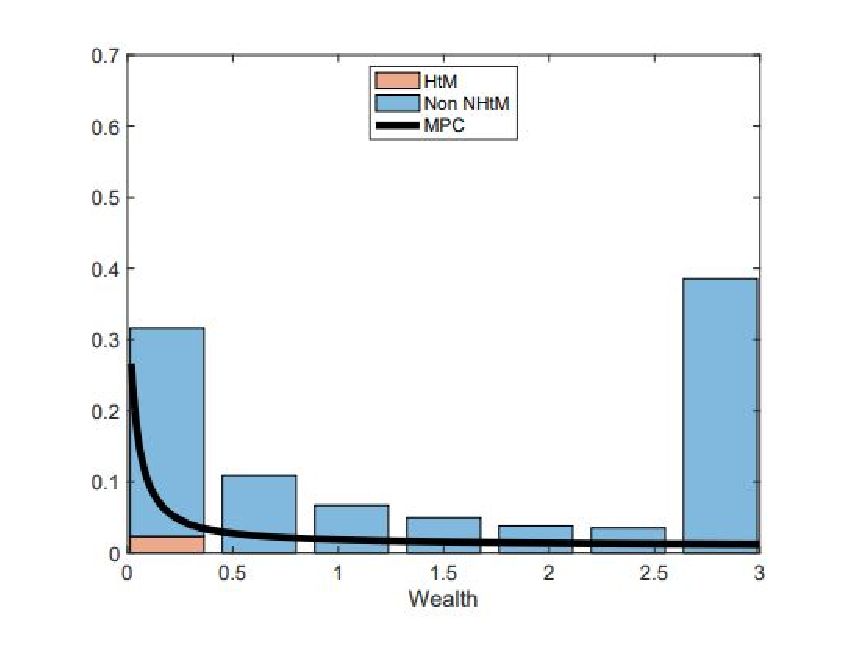
\includegraphics[width=7cm]{figs/HA-TargetMeanWealth}}
\par\end{center}
\begin{itemize}
\item High wealth target imply high $\beta$ -> HHs are very patient and
save a lot
\item Very few high MPC households
\end{itemize}
\end{frame}
%
\begin{frame}{What is a reasonable calibration of such a model?}
\begin{itemize}
\item \textbf{Calibration Strategy:}
\begin{enumerate}
\item As before, we set $\gamma=1$, so that we have log utility
\item Set the interest rate $r$ to be 1\% per year
\item Choose $\beta$ so that the model matches some target of mean wealth 
\end{enumerate}
\item \textbf{Calibration 1:}
\begin{enumerate}
\item Target US data: wealth-to-income ratio of 4.1
\item This gives an MPC of 4.6\%
\end{enumerate}
\item <+->\textbf{Calibration 2:}
\begin{enumerate}
\item Target a counterfactual wealth-to-income ratio of 0.5
\item This gives an MPC of 14\%
\end{enumerate}
\end{itemize}
\end{frame}
%
\begin{frame}{What is a reasonable calibration of such a model?}

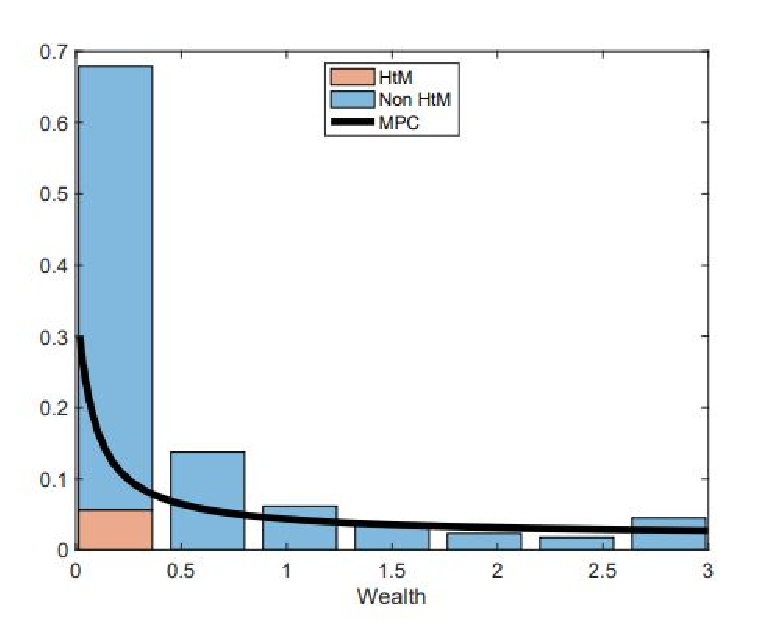
\includegraphics[width=8cm]{figs/HA-TargetLowerWealth}
\begin{itemize}
\item Now we have a lot more high MPC households (hand-to-mouth HHs)
\item But we miss the vast majority of wealth in the economy
\end{itemize}
\end{frame}
%
\begin{frame}{Main Takeaways for the MPC}
\begin{itemize}
\item <+->Can macro models generate a high MPC, and if so, how?
\begin{enumerate}
\item RA model: No 
\item One-asset HA model: only by neglecting the majority of wealth\vfill
\end{enumerate}
\item <+->Where do we go from here?
\item <+->Wanted: a version of the HA model that:
\begin{enumerate}
\item Generates a large aggregate MPC
\item Matches wealth holdings as in the data\vfill
\end{enumerate}
\item <+->Observation: 
\begin{enumerate}
\item Not all household wealth is \uline{immediately} available for consumption
smoothing
\item <+->Important difference between liquid (i.e. bank deposits) and
illiquid wealth (i.e. housing, retirement accounts)
\item <+->$\Rightarrow$ Third generation of consumption-saving models:
Multiple-asset buffer-stock consumption models
\end{enumerate}
\end{itemize}
\end{frame}
%
\begin{frame}{Two-Asset HA Model - Kaplan \& Violante (2014)}
\begin{itemize}
\item <+->Continuum of households 
\item <+->Life-cycle - HHs live for a fixed number of periods (no infinite
horizon)
\item <+->Face uninsurable idiosyncratic income shocks 
\item <+->Choose consumption, saving and \uline{portfolio allocation} 
\item <+->Two assets: liquid ($m$) and illiquid ($a$) with $r^{a}>r^{m}$ 
\begin{itemize}
\item Liquid: cash + deposits + directly held stock - unsecured debt 
\item Illiquid: housing equity + retirement account (85\% of net worth) 
\end{itemize}
\item <+->Fixed transaction cost $\kappa$ to move funds into / out of
illiquid account 
\item <+->\textbf{Q: }Why do HHs want to hold liquid or illiquid assets
in this model? Why would you want to hold both assets?
\end{itemize}
\end{frame}
%
\begin{frame}{Two-Asset HA Model}
\begin{itemize}
\item <+->Value function in period $j$ is the max of the value if you
do not ($N$) or do adjust ($A$) illiquid assets
\[
V_{j}\left(a_{j-1},m_{j-1},z_{j}\right)=max\left\{ V_{j}^{N}\left(a_{j-1},m_{j-1},z_{j}\right),\;V_{j}^{A}\left(a_{j-1},m_{j-1},z_{j}\right)\right\} 
\]
\item <+->Value function if you do not adjust:
\[
\begin{aligned}V_{j}^{N}\left(a_{j-1},m_{j-1},z_{j}\right)= & \max_{c_{j},m_{j}}u\left(c_{j}\right)+\beta\mathbb{E}_{j}\left[V_{j+1}\left(a_{j},m_{j},z_{j+1}\right)\right]\\
 & \text{ subject to }\\
 & c_{j}+m_{j}\leq m_{j-1}\left(1+r^{m}\right)+y_{j}\left(z_{j}\right)\\
 & a_{j}=a_{j-1}(1+r^{a})\\
 & m_{j}\geq\underline{m}
\end{aligned}
\]
\item <+->States: $\left(a_{j-1},m_{j-1},z_{j}\right)$ = illiquid assets,
liquid assets, productivity
\item <+->Choices: $\left(c_{j},m_{j}\right)$ = consumption, liquid asset
tmrw
\end{itemize}
\end{frame}
%
\begin{frame}{Two-Asset HA Model}
\begin{itemize}
\item Value function if you adjust:
\[
\begin{aligned}V_{j}^{A}\left(a_{j},m_{j-1},z_{j}\right)= & \max_{c_{j},a_{j},m_{j}}u\left(c_{j}\right)+\beta\mathbb{E}_{j}\left[V_{j+1}\left(a_{j},m_{j},z_{j+1}\right)\right]\\
 & \text{ subject to }\\
 & c_{j}+a_{j}+m_{j}\leq a_{j-1}(1+r^{a})+m_{j-1}(1+r^{m})-\kappa+y_{j}\left(z_{j}\right)\\
 & a_{j}\geq0,m_{j}\geq\underline{m}
\end{aligned}
\]
\vfill
\item Choices: $\left(c_{j},a_{j},m_{j}\right)$ = consumption, illiquid
asset tmrw, liquid asset tmrw
\end{itemize}
\end{frame}
%
\begin{frame}{Result: Two different Euler equations}
\begin{itemize}
\item <+->Short-Run Euler Equation - governed by saving vs dissaving in
the liquid asset (HHs adjust liquid assets every period)
\[
u'(c_{j})=\beta(1+r^{m})u'(c_{j+1})
\]
\vfill
\item <+->Long-Run Euler Equation - governed by saving vs dissaving in
the illiquid assets (only adjust illiquid asset infrequently)
\[
u'(c_{j})=\beta(1+r^{a})^{N}u'(c_{j+N})
\]

\begin{itemize}
\item where $N$ is the number of periods between adjustment
\end{itemize}
\end{itemize}
\end{frame}
%
\begin{frame}{Stylized example 1 - policy function}
\begin{itemize}
\item Zoom in on life-cycle dynamics of savings and portefolio choice in
simplified model with:
\begin{itemize}
\item Coarse hump-shaped earnings profile over life
\item Large transaction cost $\kappa$
\end{itemize}
\end{itemize}
\end{frame}
%
\begin{frame}{Stylized example 1}

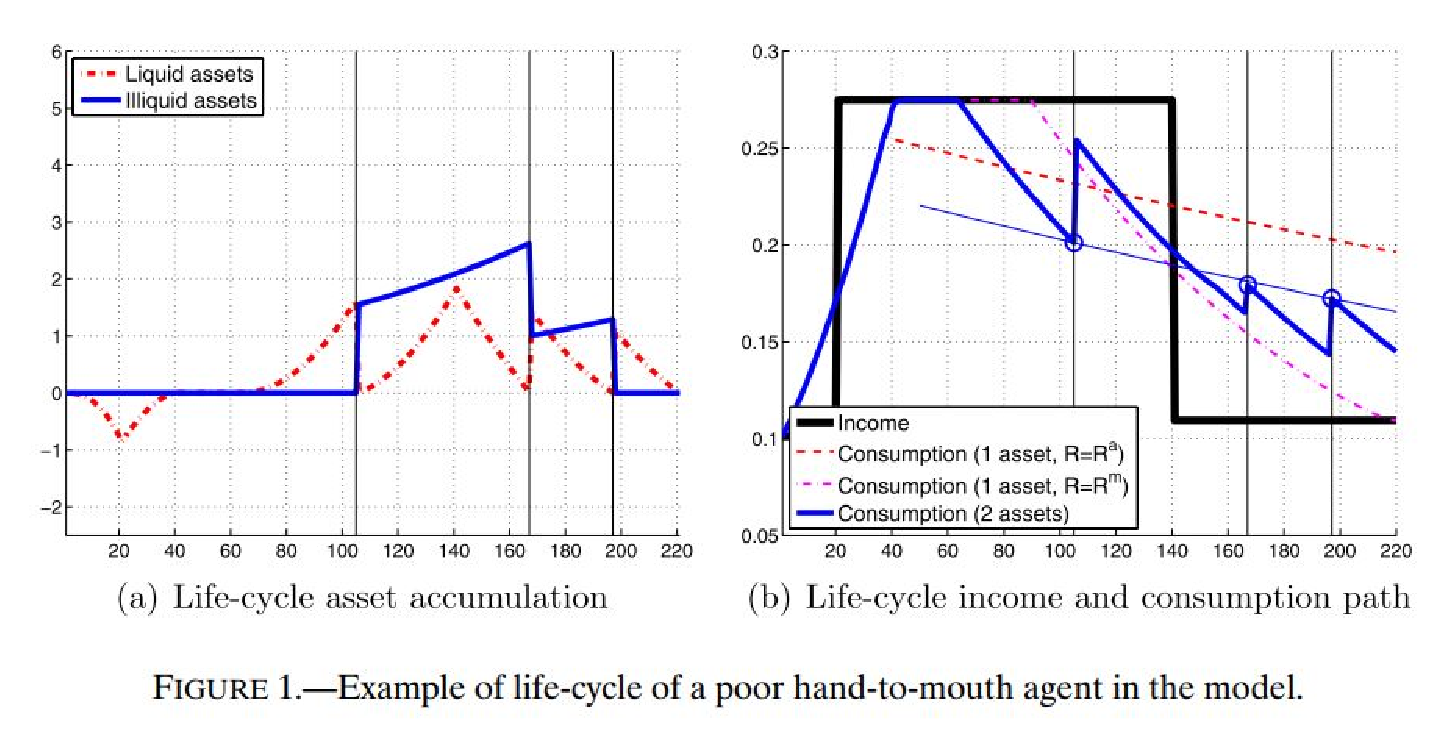
\includegraphics[width=0.8\paperwidth]{figs/PHtM-HH}

\begin{itemize}
\item 
\only<1>{Income profile: High earnings while working, lower after retirement}  
\only<2>{Liquid assets adjust more throughout lifecycle since they are suitable for consumption smoothing }  
\only<3>{Illiquid assets adjust only 3 times}  
\only<4>{Slope of consumption function \textit{between} adj. dates obey short-run Euler, slope across adj. dates obey long-run euler}  
\only<5>{Agent exhibits poor hand-to-mouth behavior between periods 40-60, when she consumes all of her income and holds zero liquid assets}  
\end{itemize}
\end{frame}
%
\begin{frame}{Example 2}

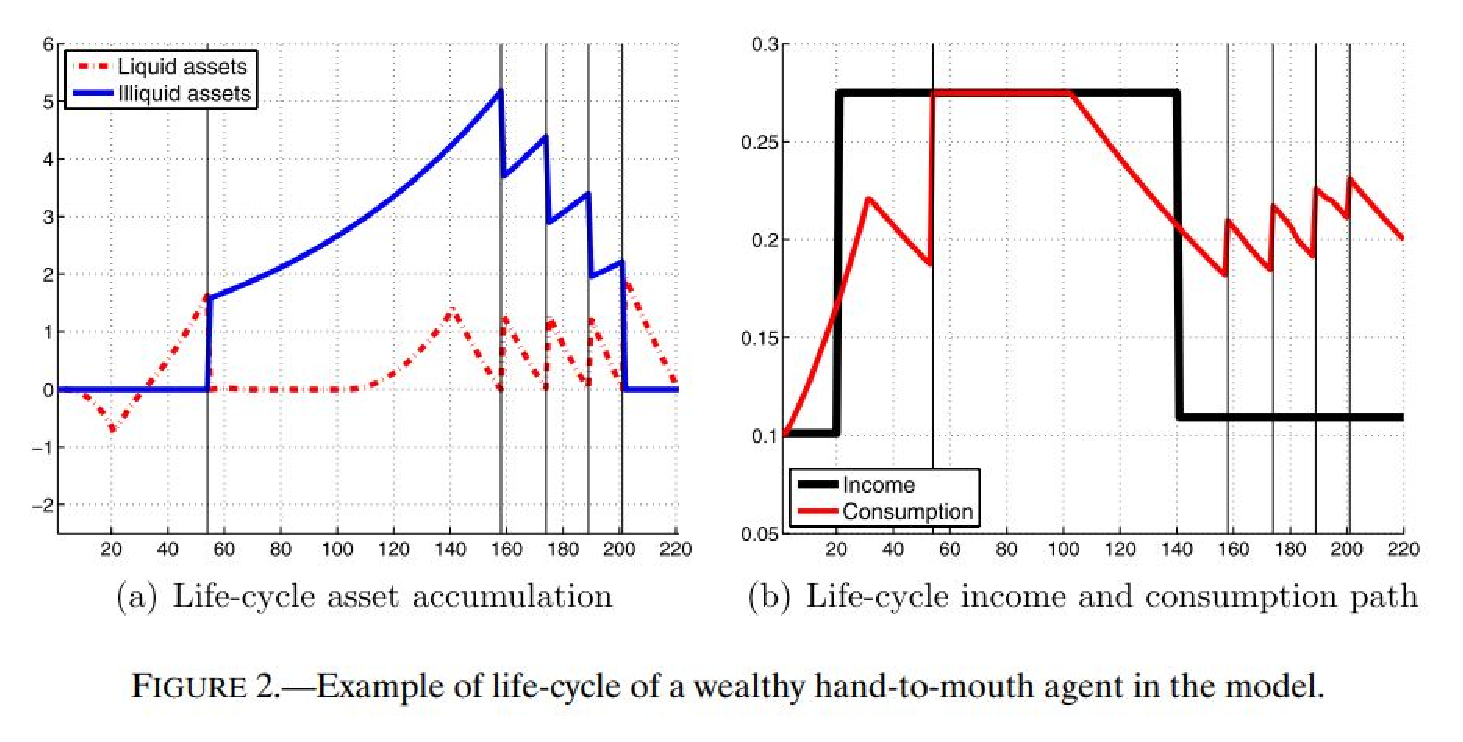
\includegraphics[width=0.8\paperwidth]{figs/WHtM-HH}

\begin{itemize}
\item 
\only<1>{Same example as before, but increase the return on the illiquid asset $r^a$. This incentivizes HHs to substitute from the liquid to illiquid asset}  
\only<2>{Agent exhibits wealthy hand-to-mouth behavior between periods 55 to 100, when she owns illiquid wealth, but zero liquid wealth}  
\end{itemize}
\end{frame}
%
\begin{frame}{Result: Emergence of Wealthy HtM Households }
\begin{itemize}
\item <+->Three types of households in the model: 
\begin{itemize}
\item Unconstrained (60\%) (positive liquid and illiquid wealth) 
\item Poor HtM: zero net worth (14\%) (zero liquid and illiquid wealth)
\item Wealthy HtM (26\%) (zero liquid wealth, but positive illiquid wealth)
\end{itemize}
\item <+->Why hold zero liquid and some illiquid wealth at the same time? 
\item <+->Trade-off between higher return and illiquidity: 
\begin{itemize}
\item Long-run gain: higher level of consumption 
\item Short-run cost: worse consumption smoothing 
\end{itemize}
\item <+->If gains exceeds costs $\Longrightarrow$ Wealthy HtM
\end{itemize}
\end{frame}
%
\begin{frame}{Wealthy HtM households in the data}
\begin{center}
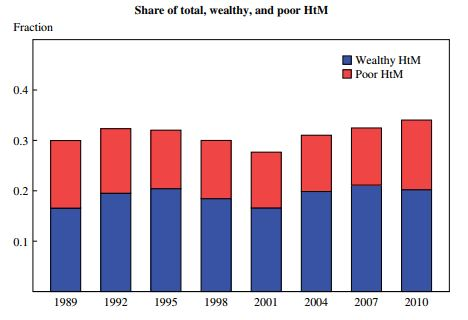
\includegraphics[width=0.6\paperwidth]{figs/HtM-by-year}\\
\par\end{center}
\begin{itemize}
\item Share of US population that are Hand-to-mouth in \emph{Survey of Consumer
Finances}
\end{itemize}
\end{frame}
%
\begin{frame}{Wealthy HtM households in the data}
\begin{center}
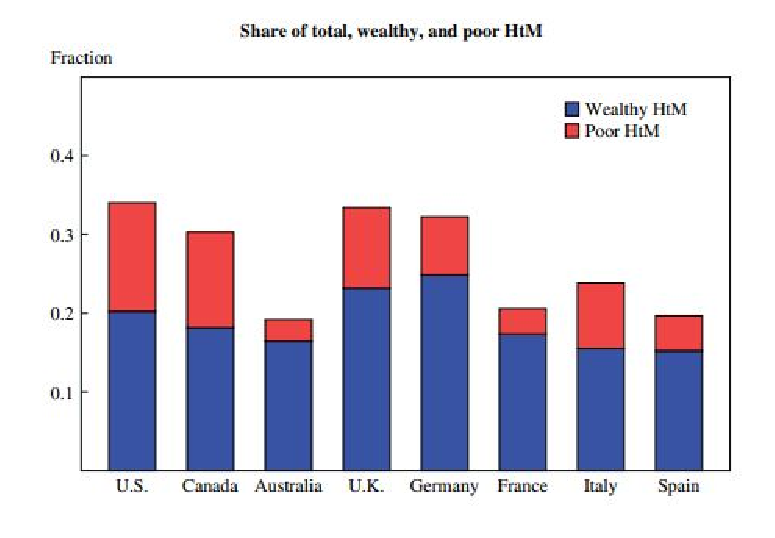
\includegraphics[width=0.7\paperwidth]{figs/HtM-by-country}
\par\end{center}

\end{frame}
%
\begin{frame}{What is a reasonable calibration of such a model?}
\begin{itemize}
\item \textbf{Calibration Strategy:}
\begin{itemize}
\item As before, we set $\gamma=1$, so that we have log utility
\item <+->Set the interest rate $r^{liq}$ on liquid assets to -2\% per
year (cash or bonds)
\item <+->There remains three parameters:
\begin{itemize}
\item Discount rate $\beta$
\item Return on illiquid assets $r^{illiq}$
\item Transaction cost $\kappa$
\end{itemize}
\item <+->Choose these three parameters so the model matches three targets:
\begin{itemize}
\item Mean wealth-to-income ratio (4.1) 
\item Share of HtM households (34\%)
\item Share of wealthy HtM households (25\%)
\end{itemize}
\end{itemize}
\end{itemize}
\end{frame}
%
\begin{frame}{Results from the two-asset model}

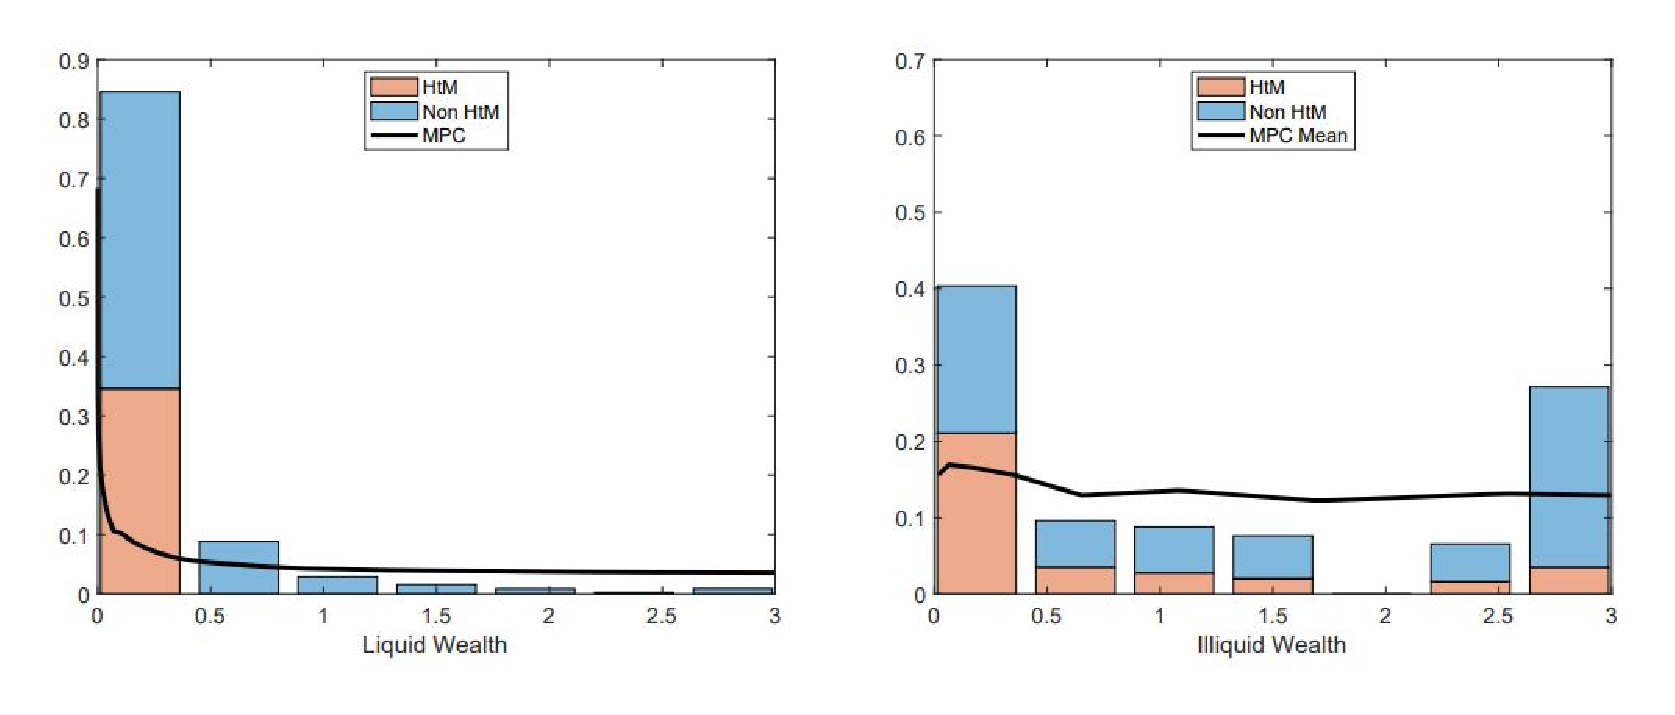
\includegraphics[width=0.9\paperwidth]{figs/HA-TwoAsset}
\begin{itemize}
\item What matters most for the MPC is liquid wealth, not total wealth
\item MPC remains high even for households with sizeable illiquid wealth
\item We can match both MPC and aggregate stock of wealth in the two-asset
model
\end{itemize}
\end{frame}
%
\begin{frame}{One-asset model with $\beta$-heterogeneity}
\begin{itemize}
\item Two-asset models a la Kaplan \& Violante (2014) are computationally
intensive to solve due to:
\begin{itemize}
\item Large state space (two endogenous states)
\item Non-convexities 
\end{itemize}
\item <+->Simpler model that still matches 1) aggregate wealth, 2) aggregate
MPC: \textbf{Heterogeneous $\beta$ model}
\item <+->Other options:
\begin{itemize}
\item Wealth-in-utility (Michaillat and Saez 2021)
\item Behavoiral models (Present Bias, Maxted et al. 2014)
\end{itemize}
\end{itemize}
\end{frame}
%
\begin{frame}{One-asset model with $\beta$-heterogeneity}
\begin{itemize}
\item <+->Standard one-asset model with \emph{ex-ante} (=permanent) preference
heterogeneity
\item <+->Discount factors $\beta$ uniformely distributed between $\left[\overline{\beta}-2\Delta,\overline{\beta}+2\Delta\right]$
(with $\Delta=0$ we obtain standard model)
\[
\begin{aligned}V\left(a_{t-1},z_{t},\beta\right)= & \max_{c_{t}}u\left(c_{t}\right)+\beta\mathbb{E}\left[V\left(a_{t},z_{t+1},\beta\right)\right]\\
 & \text{ subject to }\\
 & c_{t}+a_{t}\leq a_{t-1}\left(1+r\right)+z_{t}\\
 & a_{t}\geq0
\end{aligned}
\]
\item <+->Calibrate average $\beta$ and dispersion $\Delta$ to match
aggregate wealth and aggregate MPC
\item <+->Can match
\begin{itemize}
\item Aggregate wealth since high $\beta$ households hold a lot of wealth 
\item Aggregate MPC since low $\beta$ households have high MPC 
\end{itemize}
\end{itemize}
\end{frame}
%
\begin{frame}{One-asset model with $\beta$-heterogeneity}

\centering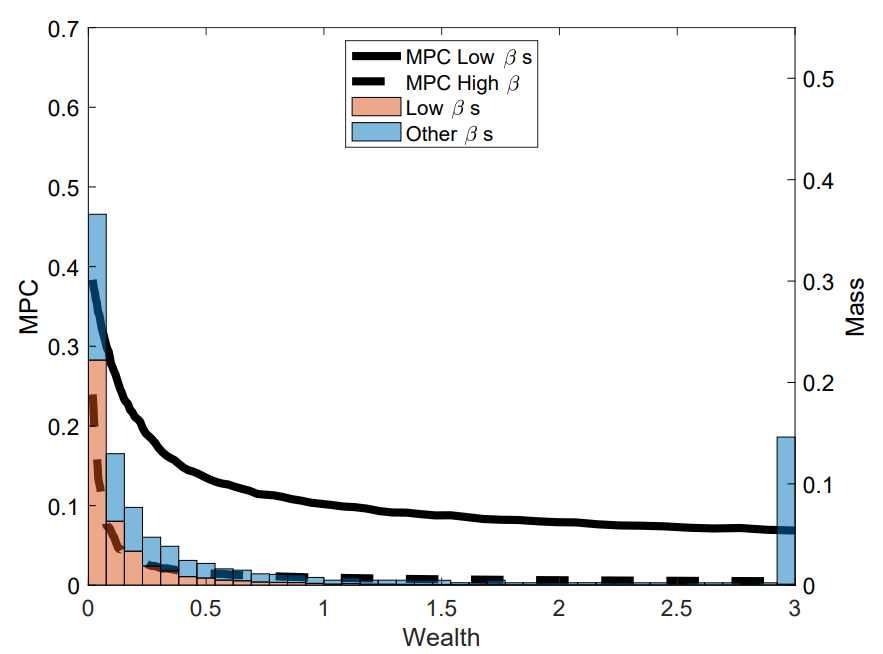
\includegraphics[width=7cm]{figs/HA-TargetMeanWealth-beta-het}
\begin{itemize}
\item Patient (high $\beta)$ households have low MPCs but hold a lot of
wealth
\item Impatient (low $\beta)$ households have high MPCs but hold a little
wealth
\end{itemize}
\end{frame}
%
\begin{frame}{Main Takeaways for the MPC}
\begin{itemize}
\item Can macro models generate a high MPC, and if so, how?
\begin{itemize}
\item RA model: No. 
\begin{itemize}
\item MPC \textasciitilde = 0.5\%
\end{itemize}
\item One-asset HA model: 
\begin{itemize}
\item Realistic wealth calibration: MPC = 4.6\%
\item Low wealth calibration or $\beta$-het: MPC = 15\%
\end{itemize}
\item Two-asset HA model: 
\begin{itemize}
\item Realistic wealth calibration: MPC = 15\%
\end{itemize}
\end{itemize}
\end{itemize}
\end{frame}
%

\section{Unemployment Risk }
\begin{frame}{Unemployment Risk and Consumption Dynamics}
\begin{itemize}
\item <+->\textbf{Question:} How does unemployment risk affect household
spending?
\begin{itemize}
\item During recessions, unemployment risk increases 
\item This may induce HHs to increase their buffer stock of assets (precautionary
savings)
\item The resulting fall in consumption may increase output volatility (note:
general equilibrium, so not today)
\item This channel has been difficult (if not impossible) to capture with
RA models
\end{itemize}
\item <+->\textbf{Our goal:} Study a HA model that can capture this channel
\begin{itemize}
\item We will closely follow Harmenberg and Öberg (2021)
\end{itemize}
\end{itemize}
\end{frame}
%
\begin{frame}{Model}
\begin{itemize}
\item <+->Start with a standard buffer stock model, expanded to have:
\begin{enumerate}
\item Durable ($d$) and nondurable consumption ($c$)
\begin{itemize}
\item Durable consumption: Car, fridge, furniture etc.
\item Nondurable consumption: Food, services etc.
\end{itemize}
\item Time varying unemployment risk\vfill
\end{enumerate}
\item <+->Households maximize
\[
\begin{aligned}\max_{\left\{ c_{it},d_{it},a_{it}\right\} _{i=0}^{\infty}}E_{0}\sum_{t=0}^{\infty}\beta^{t}u\left(c_{it},d_{it}\right)\end{aligned}
\]
\item <+->Subject to
\[
\begin{aligned}c_{t}+d_{t}+a_{t} & \leq\Upsilon\left(z_{t},n_{t}\right)+(1-\delta)d_{t-1}+Ra_{t-1}-F\left(d_{t},d_{t-1}\right),\\
a_{t} & \geq0.
\end{aligned}
\]
\end{itemize}
\end{frame}
%
\begin{frame}{Model}
\begin{itemize}
\item <+->Adjustment costs to durable consumption
\[
F\left(d_{t},d_{t-1}\right)=\left\{ \begin{array}{cl}
0 & \text{ if }d_{t}=(1-\delta)d_{t-1},\\
hd_{t-1} & \text{ if }d_{t}\neq(1-\delta)d_{t-1}
\end{array}\right.
\]
\item <+->Why do we need the adjustment cost? $\Rightarrow$ Want to capture
>>lumpy<< investment behavoir (durable purchases are infrequent,
but large)
\item <+->Income depends on both productivity and employment status
\[
\Upsilon\left(z_{t},n_{t}\right)=z_{t}\left(n_{t}+b\left(1-n_{t}\right)\right)
\]

\begin{itemize}
\item with $b<1$ = replacement rate (income when $n_{t}=0$)
\end{itemize}
\item <+->Where the employment process for $n_{t}$ is governed by two
parameters:
\begin{itemize}
\item The job \emph{finding} probability and job \emph{separation} probability
\end{itemize}
\item <+->Job separation probability = 1\% in expanisions and 2\% in recessions
\item <+->Job finding probability = 2\% in both expansions and recessions
\end{itemize}
\end{frame}
%
\begin{frame}{How might unemployment risk affect consumption}
\begin{itemize}
\item <+->Two channels:
\begin{itemize}
\item Unemployment-risk channel (ex-ante)
\item Unemployment channel (ex-post)
\end{itemize}
\item <+->What is the difference between the two channels?
\begin{itemize}
\item The first captures the saving response to an increase in future job
separation probability
\begin{itemize}
\item Increased unemployment-risk $\Longrightarrow$ larger optimal buffer
stock 
\end{itemize}
\item The second captures the fall in consumption induced by being hit by
a bad shock
\begin{itemize}
\item Decreased income $\Longrightarrow$ less resources available for consumption
\end{itemize}
\end{itemize}
\item <+->Which of these channels is more important?
\end{itemize}
\end{frame}
%
\begin{frame}{Results}

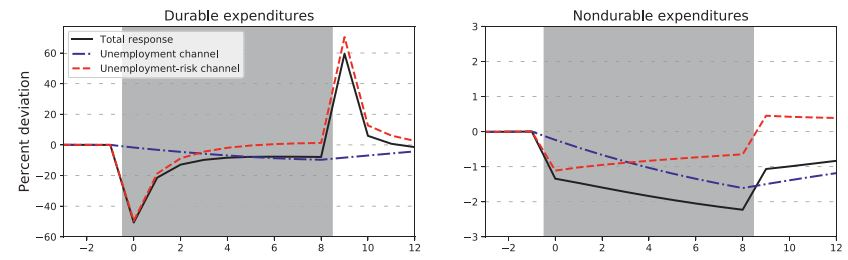
\includegraphics[width=0.8\paperwidth]{figs/Harmenberg-Oberg}
\begin{itemize}
\item <+->Response of durables is much larger than nondurables
\item <+->For durables: unemployment-risk channel is most important (\emph{wait-and-see}
effect)
\item <+->For nondurables: unemployment-risk matters initially, but unemployment
accounts for the majority in the long-term
\end{itemize}
\end{frame}
%

\section{Summary}
\begin{frame}{Summary and next week}
\begin{itemize}
\item <+->\textbf{Today: }Three applications of dynamic programming to
understand household spending dynamics
\begin{enumerate}
\item The role of credit constraints
\item Modeling the large average MPC to income shocks
\item Consumption dynamics with time-varying unemployment risk\vfill
\end{enumerate}
\item <+->\textbf{Next week: }General equilibrium
\item <+->\textbf{Homework exercises: }(see notebook in Github repo)
\begin{enumerate}
\item Adjust the discount factor, $\beta$, to target different levels of
average wealth. How does the average MPC change across calibrations?
\item Extend the model with permanent discount factor heterogeneity. Can
you find a level of dispersion that allows you to both match a high
level of liquidty and a higher MPC?
\end{enumerate}
\end{itemize}
\end{frame}
%

\end{document}
